\documentclass[final]{svjour2}
\usepackage{graphicx}
\usepackage{rotating}
\usepackage{amssymb}
\usepackage{wrapfig}
\usepackage{subfig}
\usepackage{amsmath}
\usepackage{mathptmx}
\usepackage[numbers]{natbib}
\usepackage[table]{xcolor}
\usepackage{tabularx}
\usepackage{multirow}
\usepackage{booktabs}
\usepackage{threeparttable}

\providecommand{\e}[1]{\ensuremath{\times 10^{#1}}}

%\usepackage[nofighead,nomarkers]{endfloat}
\makeatletter
\journalname{Journal of Low Temperature Physics}
%%%%%%%%%%%%%%%%%%%%%%%%%%%%%% Textclass specific LaTeX commands.


%%%%%%%%%%%%%%%%%%%%%%%%%%%%%% User specified LaTeX commands.
\bibpunct{}{}{,}{s}{}{,}

\begin{document}

\newcommand{\hdblarrow}{H\makebox[0.9ex][l]{$\downdownarrows$}-}
\title{Sub-Kelvin Thermal Conductivity and Radioactivity of Some Useful Materials in Low Background Cryogenic Experiments}

\author{N. Kellaris \and M. Daal \and E. Kramer \and M. Epland \and M. Pepin \and O. Kamaev \and P. Cushman \and B. Sadoulet \and N. Mirabolfathi \and S. Golwala \and M. Runyan}

\institute{Department of Physics, University of California, Berkeley\\ Berkeley, CA 94720, USA\\
\email{nicholaskellaris@berkeley.edu}}

\date{XX.XX.20XX}

\maketitle


\begin{abstract}
     We present measurements of the thermal conductivity for thermally isolating materials between 0.05K and 1K, as well as radioactive contamination levels. TiMet Ti 15-3-3-3, Mersen grade 2020 graphite, Vespel SP-1, SP-22, SCP-5000, and SCP-5050, Graphlite CFRP, and a Kapton/epoxy composite are all investigated. Thermal conductivities were measured using a single-heater longitudinal heat flow method. Material radioactivity was determined for the materials at a low background counting facility using a gamma detector and GEANT4-MC simulations.


\keywords{thermal conductivity, radioactivity, low temperature, Ti 15-3-3-3, Vespel, graphite, CFRP, Kapton}

\end{abstract}

\section{Introduction}
Low temperature detector experiments often require materials with low thermal conductivity and -- in the case of low background experiments such as dark matter and double-beta decay -- low radioactivity. A literature search often comes up short when it comes to sub-Kelvin thermal conductivity measurements, and low level radioactivity is seldom mentioned. We present thermal conductivity and radioactivity data for some materials which may prove useful for cryogenic experiments. TiMet Ti 15-3-3-3, Mersen grade 2020 graphite, Vespel SP-1, SP-22, SCP-5000, and SCP-5050, Graphlite CFRP, and a Kapton/epoxy composite were tested. Not all materials were tested for both thermal conductivity and radioactivity.

\section{Materials Tested}
Four types of DuPont Vespel polyimide were tested: SP-1, SP-22, SCP-5000, and SCP-5050.  Vespel SP-1 is unfilled polyimide, while SP-22 is filled polyimide base (SP-1) with 40\% graphite by weight. SCP-5000 and SCP-5050 are the newer analogs of SP-1 and SP-22 respectively; they have improved dimensional stability and strength over the SP series. All were purchased from Curbell Plastics.

Two grades of graphite were tested. The first was Mersen grade 2020, a nuclear grade graphite with grain sizes of 15$\mu$m and bulk density od 1.77g/cm$^3$. The second was POCO AXM-5Q graphite -- a highly isotropic (grain size of 5$\mu$m) industrial grade graphite with a bulk density of 1.73g/cm$^3$.

We tested TiMetal Ti 15-3-3-3, a titanium alloy with composition 15V-3Al-3Cr-3Sn by weight with Titanium as a balance. It is a meta-stable beta alloy with a superconducting transition at 3.89K. The sample was a 0.84 mil thick foil purchased from Arnold Magnetic Technologies.

A pultruded carbon-fiber composite made by Avia Sport Composites -- called Graphlite -- was tested. This is a unidirectional material with fibers nearly uniformly oriented along the pultrusion axis of the rod. Thermal conductivity was measured for a 0.156 inch rod with standard modulus material parallel to the fiber axis.

The last material measured was a Kapton-epoxy composite provided by Tech-Etch. The sample was 1 mil epoxy adhesive (pre-cured) on a 1 mil Kapton sheet. Thermal conductivity was measured parallel to the plane of the sheet. This is the same material that Tech-Etch uses in its laminated flex-circuits.

\section{Radioactivity of Samples}
The radioactive contamination of our samples was determined for five long-lived radioisotopes: U-238, Th-232, Co-60, K-40, and Cs-137. These were measured using Gopher -- a high-purity gamma detector located in the Soudan Underground Laboratory. Gamma events were counted for up to 30 days for each sample, then modelled using GEANT4-MC simulations to determine contamination. The results are shown in Table \ref{radioactivity}.

We find multiple materials with low contamination levels. Notice that the contamination for Vespel SCP-5050 is significantly less than SP-22, with up to 20 times less contamination for Th-232 and 7 times less for U-238. This may be attributable to different sources for the graphite used in each grade. For graphite, both POCO and Mersen offer purification options. The graphite is placed in an atmosphere of chlorine gas pressurized above 15psi and heated to $\sim$2000$^o$C. The chlorine permeates the material and bonds with oxidizable metals to remove them from the sample. This reduced impurities from 1000ppm to $<$1.4ppm in our samples, reducing the contamination in the POCO graphite by a factor of 50. Despite purification, grade 2020 graphite still exhibited fairly high contamination levels.

\begin{table}[htb]
\centering
\begin{threeparttable}
\rowcolors{3}{gray!20}{white}
\begin{tabular}{lrrrr}
\toprule
\multirow{2}{*}{\Large{Material}} & \multicolumn{4}{c}{\large{Contamination in mBq/kg}}\\
& U-238 & Th-232 & K-40 & Cs-137 \\\toprule
2020 Graphite (p) & 3.89 $\pm$ 0.60 & 79.63 $\pm$ 2.02 & 4.10 $\pm$ 1.65 &- \\
AXM-5Q Graphite (u-p) & 117.71 $\pm$ 2.39 & 217.13 $\pm$ 3.79 & -&-  \\
AXM-5Q Graphite (p) & 0.93 $\pm$ 0.25 & 4.93 $\pm$ 0.70 & 0.96 $\pm$ 1.16 & - \\
Vespel SP-1 & -& 5.39 $\pm$ 4.80 & -&-  \\
Vespel SP-22 & 48.38 $\pm$ 4.83 & 211.10 $\pm$ 8.99 & 7.82 $\pm$ 6.09 & -\\
Vespel SCP-5050 & 7.72 $\pm$ 0.69 & 9.95 $\pm$ 0.72 & 7.26 $\pm$ 2.18 & 0.48 $\pm$ 0.26 \\
Ti 15-3-3-3 foil & 20.4 $\pm$ 1.03 & 7.97 $\pm$ 0.89 &  3.26 $\pm$ 2.14 & - \\
Graphlite CFRP & 2.79 $\pm$ 0.89 & 0.707 $\pm$ 1.39 & 24.00 $\pm$ 4.96 & -\\
\bottomrule
\end{tabular}
 \caption{{\small Activity of listed parent for each sample. For the graphites, u-p refers to unpurified stock samples, while p refers to those samples which have been purified by the method described in this section. Co-60 contamination was not found in detectable amounts for any sample, so is not shown. Notice the drastic effect purification has on radioactive contaminants as shown by AXM-5Q (p) and (u-p). }}
\label{radioactivity}
\end{threeparttable}
\end{table}

\begin{figure}[h]
\centering
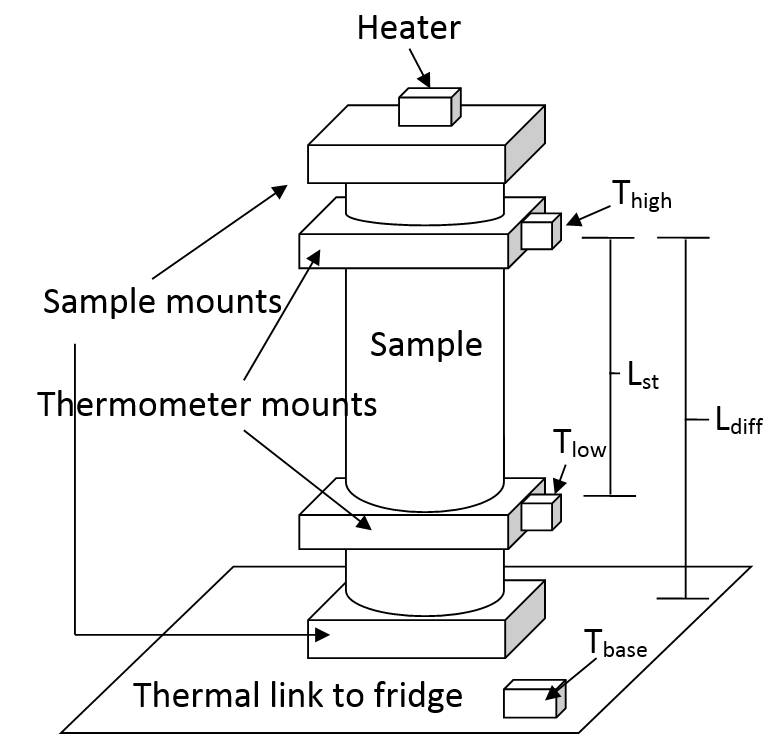
\includegraphics[width = .4\textwidth]{Rep_test_sample.png}
\qquad
\includegraphics[width = .26\textwidth]{kap_sample.png}
\includegraphics[width = 0.24\textwidth]{kap_side.png}

\caption{{\small Left shows a representative test set-up for five of the seven thermal conductivity tests. Primarily two thermometers ($T_{high}$ and $T_{low}$) were used for measurements, but a third ($T_{base}$) was mounted on the fridge end to verify base temperatures. Right shows the Kapton-epoxy and Ti 15-3-3-3 samples, which were folded back onto themselves numerous times and clamped together with the thermometer mounts to give a large cross-section.}}
\label{setup}
\end{figure}

\section{Experimental Configuration for Thermal Conductivity Tests}
The thermal conductivities of several materials were measured. All measurements were conducted in a $^3$He-$^4$He dilution refrigerator in the range of 0.05K - 1K, with the specific range varying depending on the material.

Figure \ref{setup} shows a representative test set-up for the thermal conductivity tests. A single heater was used to provide power; this was a 20k$\Omega$ metal film resistor for all tests except Vespel SP-22 and Vespel SCP-5050, which used a 2k$\Omega$ resistor. We read out temperatures with three thermometers, as shown in the figure. $T_{high}$ and $T_{low}$ were Ge thermistors, while $T_{base}$ was a RuO$_2$ thermistor, all from LakeShore\footnotemark. \footnotetext{www.lakeshore.com} A Keithley 213 Quad Voltage Source was used to read out the thermometers in a 4-wire configuration and to provide power to the heater. For temperatures above ~0.55K, a LR-700 resistance bridge was used to read out the thermometers. Thermometers were mounted on dedicated thermometer blocks which were clamped around the sample. This was intended to prevent any boundary resistance effect due to being mounted on the fridge/heater blocks. Electrical connections used 0.0012-0.003 inch diameter manganin wires, depending on the sample, all with lengths of $>$ 6 inches to the fridge thermal link.

\begin{wraptable}{r}{6.0cm}
\centering
\small
\rowcolors{3}{gray!20}{white}
\begin{tabular}{rrr}
\toprule
\textbf{Material} & $L_{st}$ (cm) & Area (cm$^2$) \\\midrule
Vespel SP-22 & 3.62 & 1.27 \\
Vespel SCP-5000 & 2.22 & 1.30 \\
Vespel SCP-5050 & 3.62 & 1.30 \\
Ti 15-3-3-3 & 3.05 & 0.91 \\
Graphlite CFRP & 4.03 & 0.12 \\
2020 graphite & 1.42 & 12.97 \\
Kapton-epoxy & 3.05 & 1.17 \\
\bottomrule
\end{tabular}
\caption{{\small Dimensions for thermal conductivity samples. $L_{st}$ refers to the center-to-center thermometer separation, as in Figure \ref{setup}. Area is the cross-section of the samples.}}
\label{dim}
\end{wraptable}

Table \ref{dim} gives the dimensions for each sample tested. Every sample was a cylindrical rod with the exception of the Ti 15-3-3-3 and Kapton-epoxy, which were strips of material folded back on itself repeatedly then clamped with the thermometer mounts, as shown in the right images of Figure \ref{setup}. Copper mounts were glued to the ends of each sample using Hardman's Double-Bubble Epoxy for the Ti 15-3-3-3, Kapton-epoxy, and grade 2020 graphite, and Stycast 1266 for all other samples. The strip samples used copper dish mounts which were flooded with epoxy to contact the sample.

\section{Thermal Conductivity Measurement Methods}
The longitudinal heat flow method was used in all tests to determine thermal conductivity. We applied a heat load to the top of the sample and let it reach equilibrium, which established a temperature gradient along the sample; this took between 30-180 minutes depending on the sample and temperature range. Once in equilibrium, we can relate power through the sample and K(T) with
\begin{equation}
P = P_{heater} + P_{parasitic} = \int_{T_{low}}^{T_{high}} \frac{A}{L_{st}} K(T)dT\\
\label{heat_flow}
\end{equation}
where A is the cross-section of the sample, $L_{st}$ is the sample length between the two thermometers (shown in Figure \ref{setup}), K(T) is the thermal conductivity of the sample, $P_{heater}$ is the power applied through the heater, and $P_{parasitic}$ is any other parasitic heat load through the sample (e.g. from wiring, voltage noise in the heater, etc.)

We primarily used two methods to determine thermal conductivity. The simplest method assumes a constant thermal conductivity\footnotemark along the gradient from $T_{high}$ to $T_{low}$. We bring thermal conductivity out of the integral, integrate with respect to T, and solve for K($T_{avg}$), where $T_{avg} = (T_{high} + T_{low})/2$. The second method assumes a parametric form for thermal conductivity -- this is often a power law at low temperatures ($K(T) = A \times T^B$). This lets us directly integrate equation \ref{heat_flow}. The free parameters are then varied to find the those values which minimize
\begin{eqnarray}
\chi^2 = \sum_{i = 1}^{n} \left[\frac{P_{total_i} - P_{expected_i}}{\sigma_{P_i}}\right]^2 \qquad ,
\label{param}
\end{eqnarray}
for n measurements, where $P_{total_i} = P_{heater_i} + P_{parasitic_i}$ is a combination of power applied to the heater and any parasitic heat loads, $P_{expected_i}$ is given by the right side of equation \ref{heat_flow}, and $\sigma_{P_i}$ is the total variance in power for a given measurement.
\footnotetext{This can be valid for gradients of $> 100$\% of $T_{avg}$ depending on the temperature dependence of the sample. See \cite{Hust1982} for details.}

\section{Thermal Conductivity Results}
Measured thermal conductivities are shown on the left of Figure \ref{plots}. Error bars are given for the points obtained using the constant thermal conductivity approximation method. The black error bars give the measurement uncertainty, while the green error bars give the combined measurement and systematic uncertainty. We also plot the parametric forms, given in Table \ref{cond_table}. The good agreement between the two methods demonstrates the validity of the constant thermal conductivity approximation. Overall errors in K(T) are estimated to be between 6\%-15\%, with the lowest temperature points being up to 20\%; these errors are heavily dominated by uncertainty in power through the sample -- especially from parasitic heat loads at low temperatures -- and on uncertainty in length for the sample; the uncertainty in length was conservatively set to the length of the thermometer mount contact area.

\begin{wraptable}{r}{5.3cm}
\centering
\small
\begin{threeparttable}
\rowcolors{3}{gray!20}{white}
\begin{tabular}{lr}
\toprule
Sample & K(T) [uW/cm-K] \\
\midrule
2020 graphite & $7.88$ T$^{1.00}$ \\
Vespel SCP-5050 & $10.0$ T$^{1.98}$ \\
Vespel SCP-5000 & $13.8$ T$^{1.11}$ \\
Vespel SP-22 & $22.1$ T$^{2.15}$ \\
Ti 15-3-3-3 & $131.1$ T$^{2.10}$ \\
Graphlite & $160.0$ T$^{1.54}$ \\
Kapton-epoxy: & \\
\multicolumn{2}{r}{$10^{1.81 + 1.01log(T) - 0.348log^2(T)}$} \\
\bottomrule
\end{tabular}
\caption{{\small Parameterized K(T) measured for materials. The Kapton-epoxy did not follow a power-law.}}
\label{cond_table}
\end{threeparttable}
\end{wraptable}

The right side of Figure \ref{plots} compares our conductivity measurements to data in the literature. We see that the thermal conductivity of grade 2020 graphite is very similar to POCO AXM-5Q. In addition, we see that both SCP-5000 and SCP-5050 are lower thermal conductivity than their counterparts SP-1 and SP-22, which makes them very interesting for experimental applications. The measured thermal conductivity for Vespel SP-22 is lower than the literature, and may be attributed to a large uncertainty in parasitic heat loads. Our measured thermal conductivity for Graphlite was higher than the literature, but still consistent. The value obtained for Kapton-epoxy is consistent with the literature as well, if we assume that the epoxy has higher thermal conductivity than Kapton. The increasing temperature dependence of Ti 15-3-3-3's thermal conductivity with decreasing temperature is not observed in our sample, but our results are consistent at higher temperatures; even so, its low thermal conductivity makes it useful for low conductance applications.

\begin{figure}[h]
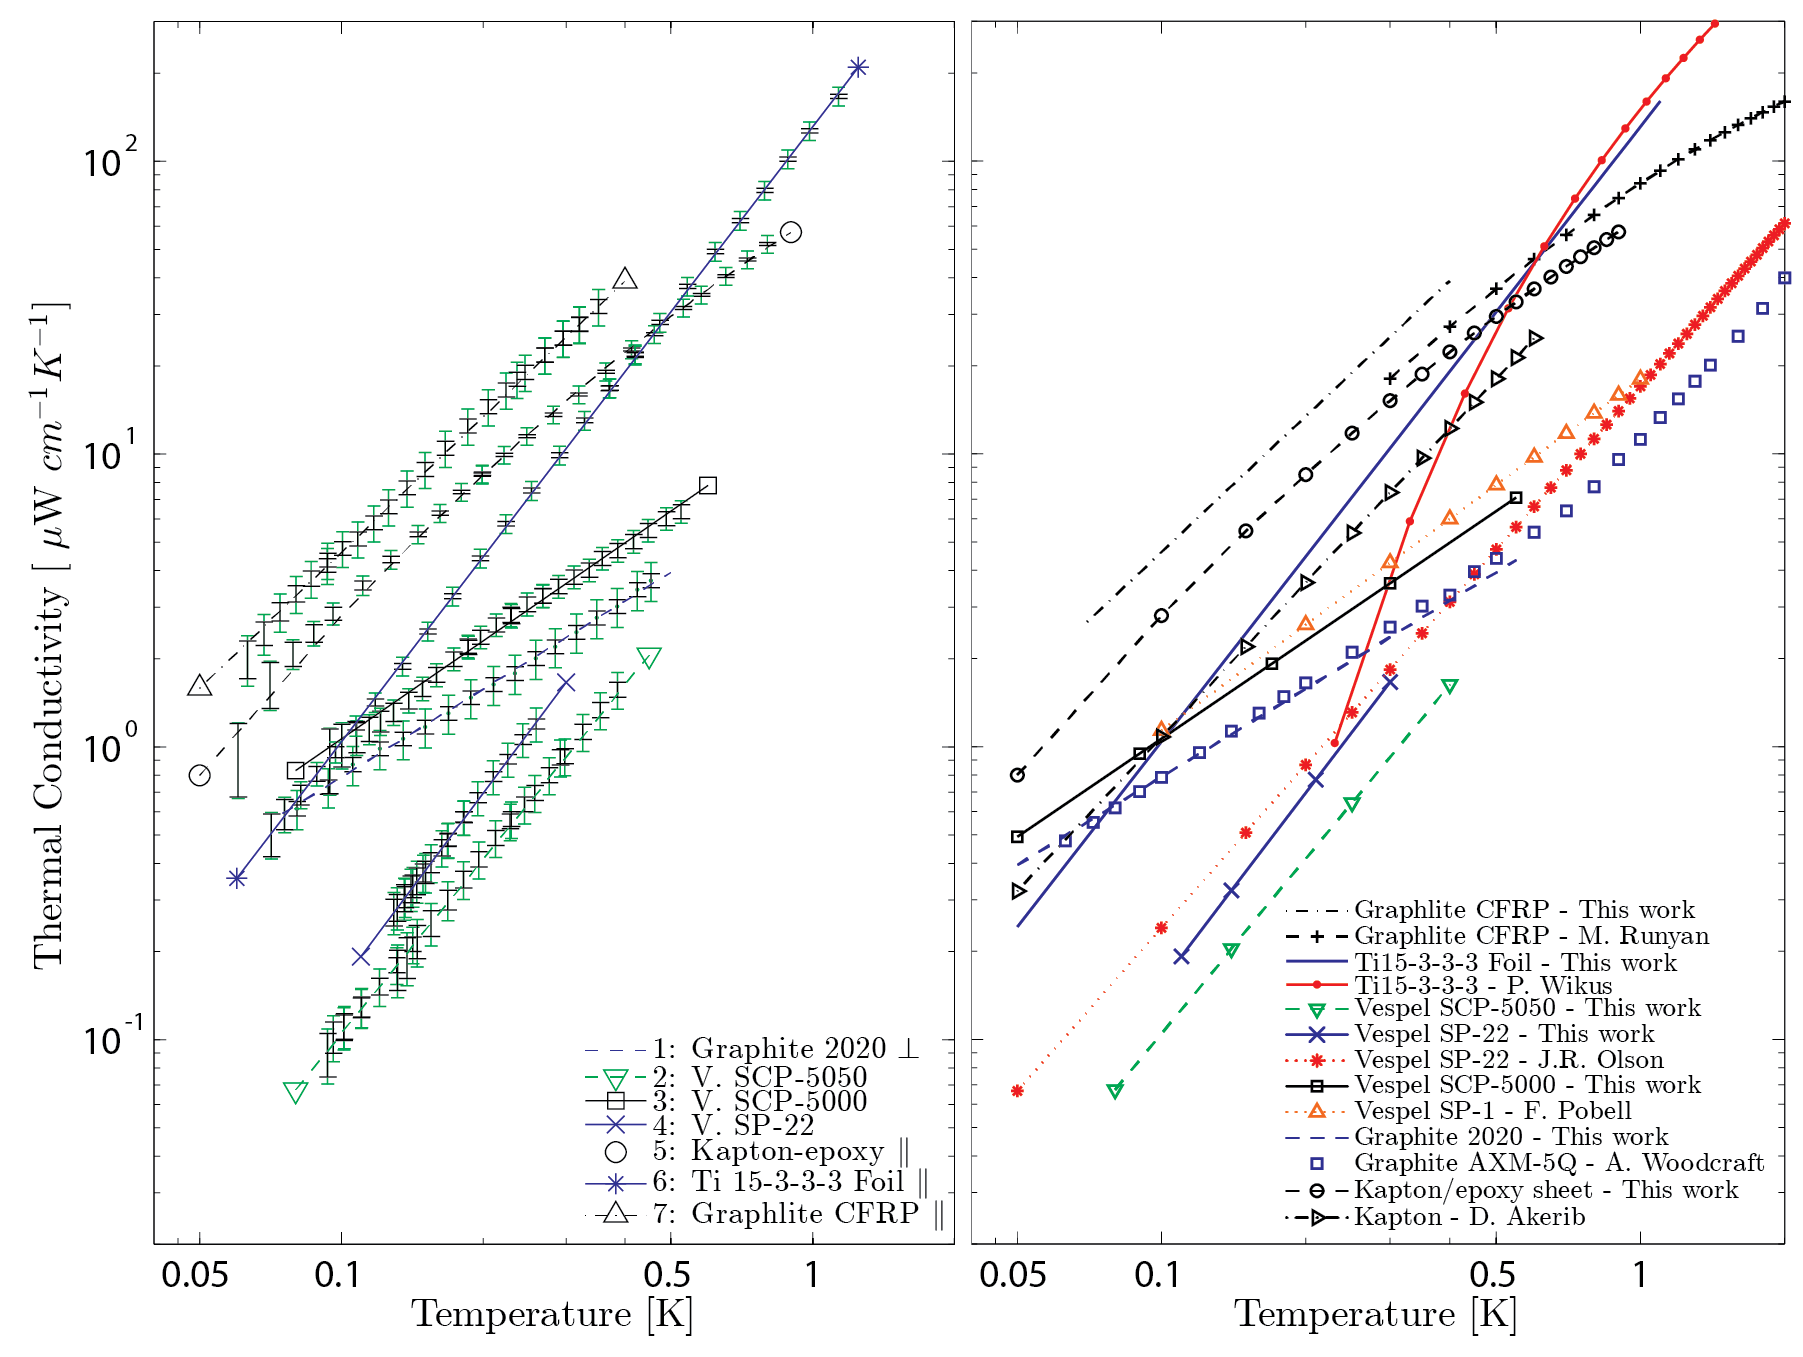
\includegraphics[width = \textwidth]{Double_plot_v2.png}
\caption{{\small Thermal conductivity of tested materials compared to other materials of interest. The $\parallel$ signifies that the Graphlite was measured parallel to the fiber axis, and the Kapton-epoxy/Ti 15-3-3-3 were measured parallel to the plane of the sheet. $\perp$ denotes that 2020 was measured perpendicular to the grain orientation. The parametric forms are plotted for data from this work. All other data is from: Graphlite\cite{Runyan2008}, Ti 15-3-3-3\cite{Wikus2010}, Vespel SP-22\cite{Olson1993}, Vespel SP-1\cite{Pobell1992}, Graphite AXM-5Q\cite{Woodcraft2009}. The Kapton data is from an in-lab measurement by Dan Akerib in the CDMS collaboration. (color version online)}}
\label{plots}
\end{figure}

\noindent \textbf{Acknowledgements}

\noindent The authors would like to thank Curbell Plastics and Tech-Etch for donating samples for testing. This work was funded by the Department of Energy and the National Science Foundation.

\begin{thebibliography}{99}

\bibitem{Hust1982}
J.G. Hust and A.B. Lankford, {\it Int. Journal of Thermophysics} \textbf{3}, 67, (1982).

\bibitem{Woodcraft2009}
A.L. Woodcraft, M. Barucci, P.R. Hastings, L. Lolli, V. Martelli, L. Risegari, and G. Ventura, {\it Cryogenics} \textbf{49}, 159, (2009).

\bibitem{Runyan2008}
M.C. Runyan and W.C. Jones, {\it Cryogenics} \textbf{48}, 448, (2008).

\bibitem{Wikus2010}
P. Wikus, S.A. Hertel, S.W. Leman, K.A. Mc{C}arthy, S.M. Ojeda, and E. Figueroa-{F}eliciano, {\it Cryogenics} \textbf{51}, 41, (2010).

\bibitem{Pobell1992}
F. Pobell, {\it Matter and Methods at Low Temperatures} (Springer--Verlag, Heidelberg, Germany, 1992)

\bibitem{Olson1993}
J.R. Olson, {\it Cryogenics} \textbf{33}, 729, (1993).

\end{thebibliography}

\end{document}
